We provide a novel approach to solve this open problem, and juxtaposes this approach and its experimental results against the current state-of-the-art models. We empirically demonstrate the separation of content and style spaces by demonstrating the inferred spaces of labelled sentences in a sentiment-transfer task, where the positive sentences in the test set are converted to equivalent sentences with a negative sentiment, and vice-versa.

This model is also generalizable using its standard implementation to problems involving multiple classes, like style transfer by authors, artists, topic etc.

Our model is built upon an autoencoder with a sequence-to-sequence (Seq2Seq) neural network \citep{sutskever2014sequence}, as described in Section \ref{ssec:seq2seq-objective}. This is the primary objective of the algorithm, whose objective function is to simply reconstruct the input text. We implement our model with both deterministic autoencoders \citep{baldi2012autoencoders} as well as variational autoencoders \citep{kingma2013auto}.

Then we introduce two auxiliary losses, multi-task loss and adversarial loss in Sections \ref{ssec:multitask-objective} and \ref{ssec:adversarial-style-objective}, respectively. In addition to these auxiliary losses, we propose a novel bag-of-words adversarial loss in Section \ref{ssec:adversarial-bow-objective}. This makes our model a dual-adversary model. Section \ref{ssec:generating-novel-text} presents the approach to transfer style in natural language generation.

Figures \ref{fig:model-overview-training} and \ref{fig:model-overview-inference} depict the training and generation processes of our approach.

\begin{figure}[ht]
	\centering
	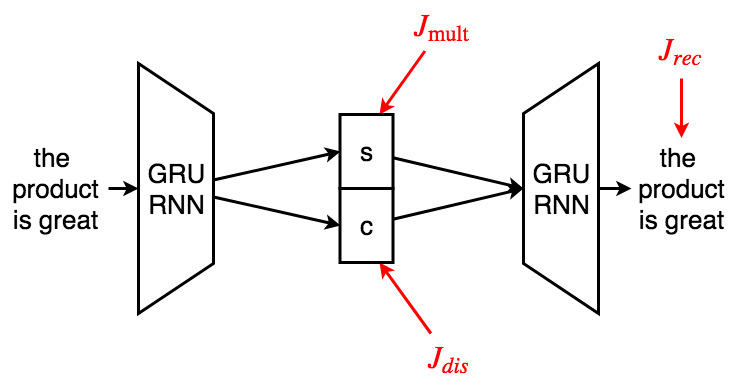
\includegraphics[width=\linewidth]{images/model-overview-training}
	\caption{Overview of Model Training}
	\label{fig:model-overview-training}
\end{figure}

\begin{figure}[ht]
	\centering
	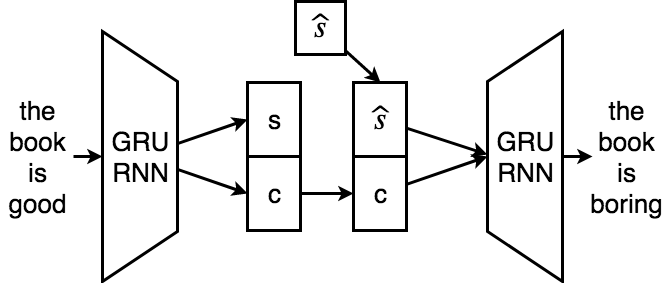
\includegraphics[width=\linewidth]{images/model-overview-inference}
	\caption{Overview of Model Inference}
	\label{fig:model-overview-inference}
\end{figure}


\section{Autoencoder} \label{ssec:seq2seq-objective}

An autoencoder encodes an input to a latent vector space, from which it decodes the input itself. By doing so, the autoencoder learns meaningful representations of data. This serves as our primary learning objective. Besides, we also use the autoencoder weights  for text generation in the attribute style-transfer application.

Let $x=(x_1, x_2, \cdots x_n)$ be an input sentence. The encoder encodes $x$ by a recurrent neural network (RNN) with gated recurrent units (GRU) \citep{cho2014learning}, and obtains a hidden state $\bm h$, which in our formulation, is two separate spaces, $\bm s$ for style and, $\bm c$ for content, which still requires an equivalent number of parameters compared to a vanilla RNN encoder.

Then a decoder RNN generates a sentence, which ideally should be $x$ itself. Suppose at a time step $t$, the decoder RNN predicts the word $x_t$ with probability $p(x_t | \bm h, x_1 \cdots x_{t-1})$, then the autoencoder is trained with cross-entropy loss, given by

First the encoder produces the style and content, given that $\theta_{E_s}$ represents the subset of encoder parameters responsible for the production of the style vector and $\theta_{E_c}$, similarly, represents the encoder responsible for the production of the content vector.
\begin{eqnarray*}
	\bm s &=& \theta_{E_s}(x) \nonumber \\
	\bm c &=& \theta_{E_c}(x) \nonumber
\end{eqnarray*}

Following which the decoder attempts to predict the original distribution of $x$ by predicting the softmax over the vocabulary size, for as many time steps as the sequence length, as shown in Equation \ref{eqn:dae-rec}
\begin{equation} \label{eqn:dae-rec}
	\mathcal{L}_\text{rec}(\bm\theta_E,\bm\theta_D)= -\mathbb{E}[log p_D(x|\bm s, \bm c)]
\end{equation}
where $\bm\theta_E$ and $\bm\theta_D$ are the parameters of the encoder and decoder, respectively.

Since this loss trains the autoencoder to reconstruct $x$, it is also called the reconstruction loss.


\subsection{Variational Autoencoder}

In addition to the deterministic auto-encoding objective presented above, we also implement a variational autoencoder. The variational sampling and KL-divergence losses are applied for both the style space $\bm s$ and the content space $\bm c$. The weights applied to each KL-divergence loss is tuned independently as a hyperparameter.

Equation \ref{eqn:vae-rec} shows the reconstruction objective that is minimized by the model in the VAE variant of our model.

\begin{eqnarray} \label{eqn:vae-rec}
	\mathcal{L}_\text{rec}(\theta_D, \theta_E; x) &=& \nonumber
	- \mathbb{E}_{q_{E_s}(\bm s|x) q_{E_c}(\bm c|x)} [log p_D(x|\bm s, \bm c)] \nonumber \\ & &
	+ \lambda_{\text{skl}} KL(q_{E_s}(\bm s|x)||p(z)) \nonumber \\ & &
	+ \lambda_{\text{ckl}} KL(q_{E_c}(\bm c|x)||p(z))
\end{eqnarray}

The motivation for using a variational autoencoder variant to compare the base deterministic autoencoder model to, is the property of VAEs to learn smooth and continuous latent spaces, without many dead zones in the latent space that cannot be sampled from. \cite{bowman2016generating} show this empirically by using the latent space of a text variational autoencoder to interpolate between and generate novel sentences from the latent spaces between two valid sentences from a corpus.

Since our objective is to use empirically inferred latent vectors to eventually achieve the attribute style transfer objective, it would be beneficial to juxtapose the experimental performance of a variational autoencoder against a deterministic autoencoder.


Besides the above reconstruction losses, we design auxiliary losses to disentangle the latent space such that $\bm h$ can be separated into two spaces $\bm s$ and $\bm c$, representing style and content respectively, i.e., $\bm h = [\bm s ; \bm c]$, where $[\cdot;\cdot]$ denotes concatenation. We also design additional regularizations on the latent space to encourage learning this disentangled representation.


\section{Multi-Task Loss} \label{ssec:multitask-objective}

Our first auxiliary loss ensures the style space does contain style information. We build a classifier trained using the style space $\bm s$ as its features, predicting the style label $y$, which is a part of the training data.

This loss can be viewed as a multi-task objective, in addition to the original reconstruction objective, which ensures that the neural network not only decodes the sentence, but also predicts its sentiment from a sub-space of the latent representation. Similar multi-task losses have been used in previous work for sequence-to-sequence learning \citep{luong2015multi}, sentence representation learning \citep{jernite2017discourse} and sentiment analysis \citep{balikas2017multitask}, among others.

In our application, we follow previous work \citep{hu2017toward,shen2017style,fu2017style} and treat the sentiment as the style of interest for our primary evaluation. However, since our model generalizes to more that one class, we uses a simple multi-layer perceptron (MLP) followed by a softmax distribution over the possible labels. The softmax function can be expressed as the following expression
\begin{equation*}
	\sigma(\mathbf{z})_j = \frac{e^{z_j}}{\sum_{k=1}^K e^{z_k}} \text{for} j \in {1, \cdots K}
\end{equation*}
where $z_j$ denotes an arbitrary label's unweighted probability and $K$ is the total number of labels in the training data. The softmax distribution is re-weighted such that it's constituent values sum up to 1, which is very useful to model probability predictions over an arbitrary number of classes.

The discriminative classification predicted distribution is given by
\begin{equation} \label{eqn:class-pred}
	p(y | \bm s; \bm\theta_\text{mult}) = softmax(\bm w_\text{mult}^\top \bm s + b_\text{mult})
\end{equation}
where $\bm\theta_\text{mult}=[\bm w_\text{mult}; b_\text{mult}]$ are the classifier's parameters for multi-task learning.

This is trained using a simple cross-entropy loss.
\begin{equation} \label{eqn:multi-task-loss}
	\mathcal{L}_\text{mult}(\bm\theta_{E};\bm\theta_\text{mult}) =
	\mathbb{E}_{y'} [\log p(y | \bm s; \bm\theta_\text{mult})]
\end{equation}
where $\bm\theta_E$ are the encoder's parameters and $y'$ is the true class distribution.


\section{Adversarial Style Discriminator} \label{ssec:adversarial-style-objective}

The above multi-task loss only operates on the style space, but does not have an effect on the content space $\bm c$. With only the multi-task loss, we cannot guarantee that the encoder would not choose to encode stylistic features within the content space.

We therefore apply an adversarial loss to disentangle the content space from style information, inspired by adversarial generation \citep{goodfellow2014generative}, adversarial domain adaptation \citep{liu2017adversarial}, and adversarial style transfer \citep{fu2017style}.

The idea of adversarial loss is to introduce an adversary that deliberately attempts to discriminate style $s$ of training samples using only the content vector $\bm c$. Then the autoencoder is trained to learn such a content vector space that its adversary cannot predict style information.

Concretely, the adversarial discriminator predicts style $y$ by using a softmax distribution over a multi-layer perceptron
\begin{equation}
	p(y | \bm c; \bm\theta_\text{dis}) = softmax(\bm w_\text{dis}^\top \bm c + b_\text{dis})
\end{equation}
where $\bm\theta_\text{dis}=[\bm w_\text{dis}; b_\text{dis}]$ are the parameters of the adversary.

It is trained by minimizing the following objective
\begin{equation} \label{eqn:adv-disc-loss}
	\mathcal{L}_\text{dis}(\bm\theta_{E};\bm\theta_\text{dis}) =
	\mathbb{E}_{y'} [\log p(y | \bm c; \bm\theta_\text{dis})]
\end{equation}

The adversarial loss appears similar to the multi-task loss as in Equation \ref{eqn:multi-task-loss}. However, it should be emphasized that, for the adversary, the gradient is not propagated back to the autoencoder, i.e., $\bm c$ is treated as shallow features. The only adversarial component is the loss itself. The network parameters are mutually exclusive for the autoencoder and the adversarial discriminator.

Having trained an adversary, we would like the autoencoder to learn latent representations, that $\bm c$ is not discriminative in term of the style or attribute we want to transfer. In other words, we penalize the entropy of the adversary's prediction, given by
\begin{equation}
	\mathcal{L}_\text{adv}(\bm\theta_E) = \mathcal{H}(p_\text{dis}(y | \bm c))
\end{equation}
where $\mathcal{H}=-\sum_{i\in\text{labels}} p_i\log p_i$ is the empirical Shannon entropy of the distribution. The adversarial objective is maximized, in this phase, with respect to the encoder. The motivation behind this objective is to increase the uncertainty of the discriminative classifier with respect to predicting style from the content vector. The maximum entropy value attainable over the distribution of attributes is the point at which each label is predicted with equal-probability i.e. the highest uncertainty.


\section{Adversarial Bag-of-Words Discriminator} \label{ssec:adversarial-bow-objective}

In addition to the auxiliary losses used above, we also propose a novel bag-of-words discriminator on the style space. The motivation for having this objective is to try and emulate the adversarial signal provided by the style discriminator, but and do the same for the content. Here, we define the content of the sentence as the words from the original sentence without any sentiment words.hu2004mining
hu2004mining
The input sentences $x$ are represented as a vector of the same size as the corpus vocabulary, with each index of the vector a discrete probability of a word's presence in the sentence. Therefore, this bag-of-words representation is comprised of only 1s and 0s.

The bag-of-words discriminator, uses the style vector produced by the autoencoder model and tries to predict the true bag-of-words distribution using a set of parameters that are distinct from those of the autoencoder. The discriminator uses a logistic regression to predict a probability of each words occurrence in the original sentence, between 0 and 1.
\begin{equation}
	p(b | \bm s; \bm\theta_\text{bow}) = \sigma(\bm w_\text{bow}^\top \bm s + b_\text{bow})
\end{equation}
where $b$ is the predicted bag-of-words distribution.

This objective is trained in a similar method to the style adversary, by using a cross-entropy loss
\begin{equation} \label{eqn:adv-bow-disc-loss}
	\mathcal{L}_\text{bow}(\bm\theta_{E};\bm\theta_\text{bow}) =
	\mathbb{E}_{b'} [\log p(b | \bm c; \bm\theta_\text{bow})]
\end{equation}
where $b'$ is the true distribution and can be considered part of the training data.

Similar to the style adversary, the empirical Shannon entropy of the predicted distribution is provided as a training signal for the autoencoder model to maximize.
\begin{equation}
	\mathcal{L}_\text{badv}(\bm\theta_E) = \mathcal{H}(p_\text{bow}(b | \bm s))
\end{equation}

The motivation for this adversarial loss is similar to the one used in the context of the style discriminator. We want to encourage the encoder to learn a representation of style that the bag-of-words discriminator cannot predict most of the original words from.

\subsection{Lexicon Augmented Discriminator}

An improvement to the bag-of-words discriminator could be made assuming the availability of a lexicon of words that are associated with a high probability with each of the styles that we are trying to disentangle.

The bag-of-words representation that excludes these words can now be created, such that the size of each representation is $(\text{\# vocab words}) \setminus (\text{\# lexicon words})$.

The bag-of-words adversary will not penalize the autoencoder model for encoding words that are pertinent and discriminative for style that may be encoded in the style space. For the sentiment task in our experiments, we use a lexicon of positive and negative sentiments words curated by \cite{hu2004mining}.


\section{Style Dropout Regularization} \label{ssec:style-dropout}

In addition to the regular training objectives, we also describe a novel regularization technique for disentanglement tasks. This method can also be viewed as analogous to a training objective like the bag-of-words loss.

In our formulation of the model, we describe the main adversarial loss for style disentanglement by training a discriminator on the content space. However, there is a possibility of the autoencoder learning to ignore the content vector during generation entirely and use only the style space for encoding and later decoding the salient features of the corpus. This scenario is depicted in \ref{fig:model-content-bypass} and can be thought of as the model bypassing the content space due to the presence of an adversary that penalizes any signals for style.

\begin{figure}[ht]
	\centering
	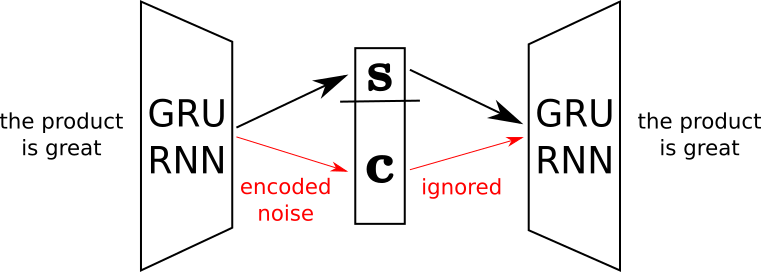
\includegraphics[width=\linewidth]{images/model-content-bypass}
	\caption{Content Space Bypassing}
	\label{fig:model-content-bypass}
\end{figure}

To address this issue, we propose a customized version of Dropout \cite{srivastava2014dropout}. Similar to how each neuron in a network is dropped out with a pre-defined probability in the general version of dropout, in this version, we drop out entire style vectors in the mini-batch randomly with a pre-defined probability. The motivation for doing this is to reinforce the fact that the content latent vector is not to ignored for the auto-encoding task despite the negative training signal from the adversary.


\section{Training Process}

The overall loss used for the autoencoder is thus comprised of four different, objectives, the reconstruction objective, the multi-task objective and the style and content adversaries.
\begin{eqnarray*}
	\mathcal{L}_\text{ovr} &=&
	\mathcal{L}_\text{rec}(\bm\theta_E, \bm\theta_D)
	+ \lambda_\text{mult}(\bm\theta_E,\bm\theta_\text{mult}) \\ & &
	- \lambda_\text{adv} \mathcal{L}_\text{adv}(\theta_E)
	- \lambda_\text{badv} \mathcal{L}_\text{badv}(\theta_E)
\end{eqnarray*}
where $\lambda_\text{mult}$, $\lambda_\text{adv}$ and $\lambda_\text{badv}$ balance these losses.

To summarize the model training setup, our training process is a loop of the minimization objectives described in Algorithm \ref{alg:training-process}.

\begin{algorithm}[H]
	\While{epochs remaining}{
		minimize $\mathcal{L}_\text{dis}(\bm\theta_\text{dis})$ w.r.t. $\bm\theta_\text{dis}$\;
		minimize $\mathcal{L}_\text{bow}(\bm\theta_\text{bow})$ w.r.t. $\bm\theta_\text{bow}$\;
		minimize $\mathcal{L}_\text{ovr}(\bm\theta_E, \bm\theta_D)$ w.r.t. $\bm\theta_E, \bm\theta_D, \bm\theta_\text{mult}$\;
	}
	\caption{\label{alg:training-process} Training Algorithm}
\end{algorithm}

We use the the Adam optimizer \citep{kingma2014adam} with an initial learning rate of $10^{-3}$ and train the model for 20 epochs. Both the autoencoder and its adversary are trained once per epoch with $\lambda_\text{mult} = 1$, and $\lambda_\text{adv} = 0.3$ and $\lambda_\text{badv} = 0.0001$.


\section{Generating Style-Transferred Sentences} \label{ssec:generating-novel-text}

A direct application of our disentangled latent space is style transfer for natural language generation. For example, we can generate a sentence with generally the same meaning (content) but an opposite sentiment.

Let $x$ be an input sentence with $\bm s$ and $\bm c$ being the encoded, disentangled style and content vectors, respectively. If we would like to transfer its content to a different style, we compute an empirical estimate of the target style's vector $\hat{\bm s}$ by
$$\hat{\bm s}=\frac{\sum_{i\in\text{target style}}\bm s_i}{\text{\# target style samples}}$$. The inferred target style $\hat{\bm s}$ is concatenated with the encoded content $\bm c$ for decoding (Figure \ref{fig:model-overview-inference}).


\subsection{Nearest-Neighbour Approach for Sentence Generation}

The inference approach described above using the empirically learned mean embedding in the style space and applies it to all future inference requirements. Though simple and intuitive, this method is fairly rigid and doesn't take into account the fact that the inference time sentences' content could vary from the acceptable content embeddings that can be coupled with the mean style embedding used.

To address this, we also propose a nearest neighbour approach to identify better candidates for the style embedding than the empirical mean of training time style embeddings. Algorithm \ref{alg:nearest-neighbour} describes our method.

\begin{algorithm}[H]
	\KwData{$S \Rightarrow$ empirical style embeddings from the training data}
	\KwData{$C \Rightarrow$ empirical content embeddings from the training data}
	\KwData{$s \Rightarrow$ inferred content embedding (singular) of a test sample}
	\KwData{$c \Rightarrow$ inferred style embedding (singular) of a test sample}
	\KwData{$N \Rightarrow$ number of neighbours (hyperparameter)}
	\KwResult{new sentence generation style vector for transferring style}
	$(S, C) \Rightarrow$ pairs of (style, content) embeddings\;
	$(\text{cosine-distance}, \text{style-vector}) \Rightarrow$ empty list of tuples\;
	\For{$s_t, c_t$ in $(S, C)$}{
		Compute $cd$, the cosine distance between $c$ and $c_t$\;
		Add tuple $(cd,s_t)$ to $(\text{cosine-distance}, \text{style-vector})$\;
	}
	$\text{best-tuples} \Rightarrow$ N best tuples with minimum cosine distance in $(\text{cosine-distance}, \text{style-vector})$\;
	define $\text{aggregate-style-vector}$\;
	\For{$cd, s_t$ in $\text{best-tuples}$}{
		Add $s_t$ to $\text{aggregate-style-vector}$\;
	}
	\KwRet{$\frac{\text{aggregate-style-vector}}{N}$}\;

	\caption{\label{alg:nearest-neighbour} Nearest-Neighbour Algorithm}
\end{algorithm}

However, this method is computationally more expensive since, for each test sentence, we need to iterate over the empirical content embeddings whose number is of the same order of magnitude as the training data.
